\documentclass{beamer}
\usetheme{Madrid}
\usepackage[utf8]{inputenc}
% \usepackage[croatian]{babel}
\usepackage{amsmath, amsfonts, amssymb}
\usepackage{float}
\usepackage{tikz, tikzscale}
\usepackage{subcaption}
\usetikzlibrary{decorations.pathmorphing}
\usetikzlibrary{positioning}
\usetikzlibrary{calc}
\usepackage{adjustbox}
\DeclareMathOperator{\Ima}{Im}

\title[$\alpha$-labeling of banana tree graphs]{\texorpdfstring{$\alpha$}{Alpha}-labeling of banana tree graphs}
\author{Borna Gojšić}
\institute{FER, University of Zagreb}
\date{September 9th 2025}

\begin{document}

\begin{frame}
  \titlepage
\end{frame}

% \begin{frame}{Sections}
%   \tableofcontents
% \end{frame}

% \section{Introduction}

% \begin{frame}{Motivation}
%   \begin{itemize}
%     \item Rosa (1967) introduced graceful ($\beta$) labeling and $\alpha$-labeling
%   \end{itemize}
% \end{frame}

\section{Basic notions and results}

\begin{frame}{Graceful labeling of a tree}
  \vspace{-0.3em}
  \begin{block}{Definition [A. Rosa, 1967.]}
    \vbox{\parindent=0pt
      \setlength\abovedisplayskip{0pt}
      \setlength\abovedisplayshortskip{0pt}
      \setlength\belowdisplayskip{0pt}
      \setlength\belowdisplayshortskip{0pt}
      We say that a labeling of a graph $G$ is \textit{graceful} if $\Ima f \subseteq [m + 1]$, the induced edge labeling $f^*: E \rightarrow \mathbb{N}$ defined by $f^*(vw) = |f(v) - f(w)|$
      is injective and   $\Ima f^* = \{ f^*(vw) \, : \, vw \in E \} = [n-1].$
    }
  \end{block}
  \vspace{-0.3em}
  \begin{block}{Example}
    \vspace{-0.4em}
    \begin{figure}[H]
      \centering
      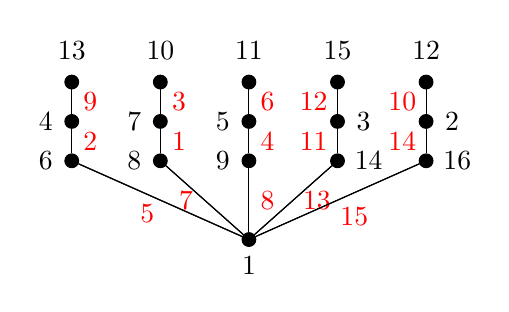
\begin{tikzpicture}[scale=0.5, every node/.style={circle, draw=black, fill=black, inner sep=1.75pt}]

        % Root node
        \node (root) at (0, -3) {};

        % Number of star graphs
        \def\nstars{5}

        % Leaves per star graph
        \def\leaves{2}

        % Radius for positioning leaves
        \def\radius{1}

        % Horizontal distance between star graphs
        \def\hstep{1.5}

        % Draw star graphs attached to the root node
        \foreach \i in {1,...,\nstars} {
          % Coordinates for the star's central node
          \node (c\i) at ({1.5*((\i-1)*\hstep - (\nstars-1)*\hstep/2)}, 0) {};

          % Draw leaves around each star node
          \foreach \j in {1,...,\leaves} {
            \node (l\i\j) at ([shift={(270 - 360/\leaves + \j*360/\leaves: \radius)}] c\i) {};
            \draw (c\i) -- (l\i\j);
          }

          % Find the lowest leaf (typically the one at 270 degrees)
          \draw (root) -- (l\i1);
        }

        \node[fill=none, draw=none, label=below:{$1$}] at (root) {};

        \node[fill=none, draw=none, label=left:{4}] at (c1) {};
        \node[fill=none, draw=none, label=left:{7}] at (c2) {};
        \node[fill=none, draw=none, label=left:{5}] at (c3) {};
        \node[fill=none, draw=none, label=right:{3}] at (c4) {};
        \node[fill=none, draw=none, label=right:{2}] at (c5) {};

        \node[fill=none, draw=none, label=left:{$6$}] at (l11) {};
        \node[fill=none, draw=none, label=above:{$13$}] at (l12) {};

        \node[fill=none, draw=none, label=left:{$8$}] at (l21) {};
        \node[fill=none, draw=none, label=above:{$10$}] at (l22) {};

        \node[fill=none, draw=none, label=left:{$9$}] at (l31) {};
        \node[fill=none, draw=none, label=above:{$11$}] at (l32) {};

        \node[fill=none, draw=none, label=right:{$14$}] at (l41) {};
        \node[fill=none, draw=none, label=above:{$15$}] at (l42) {};

        \node[fill=none, draw=none, label=right:{$16$}] at (l51) {};
        \node[fill=none, draw=none, label=above:{$12$}] at (l52) {};

        \draw (root) -- (l11) node[midway, below left, text=red, fill=none, draw=none] {$5$};
        \draw (root) -- (l21) node[midway, left, text=red, fill=none, draw=none] {$7$};
        \draw (root) -- (l31) node[midway, right, text=red, fill=none, draw=none] {$8$};
        \draw (root) -- (l41) node[midway, right, text=red, fill=none, draw=none] {$13$};
        \draw (root) -- (l51) node[midway, below right, text=red, fill=none, draw=none] {$15$};

        \draw (c1) -- (l11) node[midway, right, text=red, fill=none, draw=none] {2};
        \draw (c1) -- (l12) node[midway, right, text=red, fill=none, draw=none] {$9$};

        \draw (c2) -- (l21) node[midway, right, text=red, fill=none, draw=none] {$1$};
        \draw (c2) -- (l22) node[midway, right, text=red, fill=none, draw=none] {$3$};

        \draw (c3) -- (l31) node[midway, right, text=red, fill=none, draw=none] {$4$};
        \draw (c3) -- (l32) node[midway, right, text=red, fill=none, draw=none] {$6$};

        \draw (c4) -- (l41) node[midway, left, text=red, fill=none, draw=none] {$11$};
        \draw (c4) -- (l42) node[midway, left, text=red, fill=none, draw=none] {$12$};

        \draw (c5) -- (l51) node[midway, left, text=red, fill=none, draw=none] {$14$};
        \draw (c5) -- (l52) node[midway, left, text=red, fill=none, draw=none] {$10$};

      \end{tikzpicture}
    \end{figure}
    \vspace{-0.8em}
  \end{block}
  \vspace{-0.3em}
  \begin{block}{Conjecture [Ringel-Kotzig]}
    \vbox{\parindent=0pt
      \setlength\abovedisplayskip{0pt}
      \setlength\abovedisplayshortskip{0pt}
      \setlength\belowdisplayskip{0pt}
      \setlength\belowdisplayshortskip{0pt}
      All trees are graceful.
    }
  \end{block}
\end{frame}

\begin{frame}{$\alpha$-labeling of a tree}
  \begin{block}{Definition [A. Rosa, 1967.]}
    \vbox{\parindent=0pt
      \setlength\abovedisplayskip{0pt}
      \setlength\abovedisplayshortskip{0pt}
      \setlength\belowdisplayskip{0pt}
      \setlength\belowdisplayshortskip{0pt}
      A labeling of a graph $G$ is an \textit{$\alpha$-labeling} if it is graceful and if there exists a constant $\alpha \in \mathbb{N}$ such that
      $$ f(v) \leq \alpha < f(w) \mbox{ or }  f(w) \leq \alpha < f(v), \mbox{ for all } vw \in E.
      $$
    }
  \end{block}
  \begin{block}{Example}
    \begin{figure}[H]
      \centering
      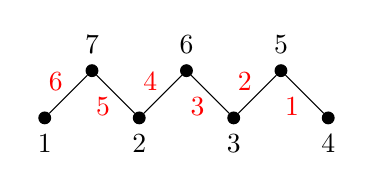
\begin{tikzpicture}[scale=0.6, every node/.style={circle, draw, fill=black, inner sep=1.5pt}]
        \def\n{7} % Change this value for different n

        % Draw the vertices
        \foreach \i in {1,...,\n} {
          % Check if \i is even or odd and set color accordingly
          \ifodd\i
          \node (v\i) at (\i,-0.5) {};
          \else
          \node (v\i) at (\i,0.5) {};
          \fi
        }

        \draw (v1) -- (v2) node[midway, above left, text=red, fill=none, draw=none] {6};
        \draw (v2) -- (v3) node[midway, below left, text=red, fill=none, draw=none] {5};
        \draw (v3) -- (v4) node[midway, above left, text=red, fill=none, draw=none] {4};
        \draw (v4) -- (v5) node[midway, below left, text=red, fill=none, draw=none] {3};
        \draw (v5) -- (v6) node[midway, above left, text=red, fill=none, draw=none] {2};
        \draw (v6) -- (v7) node[midway, below left, text=red, fill=none, draw=none] {1};

        \node[draw=none, fill=none, below=3pt] at (v1) {$1$};
        \node[draw=none, fill=none, above=3pt] at (v2) {$7$};
        \node[draw=none, fill=none, below=3pt] at (v3) {$2$};
        \node[draw=none, fill=none, above=3pt] at (v4) {$6$};
        \node[draw=none, fill=none, below=3pt] at (v5) {$3$};
        \node[draw=none, fill=none, above=3pt] at (v6) {$5$};
        \node[draw=none, fill=none, below=3pt] at (v7) {$4$};
      \end{tikzpicture}
      \caption*{$\alpha$-labeling of a tree with $\alpha = 4$}
    \end{figure}
  \end{block}
  \begin{itemize}
    \item Applications of $\alpha$-labelings: coding theory, graph decompositions
  \end{itemize}
\end{frame}

\begin{frame}{Conjugate and reverse $\alpha$-labelings}
  \begin{block}{Remark [A. Rosa, 1967.]}
    \begin{enumerate}
      \item If $f$ is an $\alpha$-labeling of $G$ and $f^*(vw) = 1$ for some $v, w \in V$, then $\alpha = \min\{f(v), f(w)\}$.
      \item If $f$ is an $\alpha$-labeling of a graph $G$ with $n$ vertices, then its complementary labeling $\overline{f}$ defined as $\overline{f}(v) = n + 1 - f(v)$ is also an $\alpha$-labeling of $G$ with $\overline{\alpha} = n - \alpha + 1$.
      \item If $f$ is an $\alpha$-labeling of $G$, its reverse (or inverse) labeling $f^r$ defined as
        $$
        f^r(v) =
        \begin{cases}
          \alpha + 1 - f(v), & f(v) \leq \alpha \\
          n + \alpha + 1 - f(v), & f(v) > \alpha
        \end{cases}
        $$
        is also an $\alpha$-labeling of $G$ with $\alpha^r = \alpha$.
    \end{enumerate}
  \end{block}
\end{frame}

\section{Banana trees}

\begin{frame}{Definition of a banana tree \( B(n, k) \)}
  \begin{itemize}
    \item Focus of our work: \textbf{$\alpha$-labeling} and a special family of trees -- banana trees
    \item Hierarchical structure: \( n \) star graphs \( S_k \)
    \item Each star is connected to a central vertex (root)
  \end{itemize}
  %   \begin{figure}[H]
  %     \centering
  %     \begin{subfigure}{0.18\textwidth}
  %       \centering
  %       \begin{tikzpicture}[scale=0.3, every node/.style={circle, draw=black, fill=black, inner sep=0.75pt}]
  %         % Number of star graphs
  %         \def\nstars{1}
  %         % Leaves per star graph
  %         \def\leaves{3}
  %         % Radius for positioning leaves
  %         \def\radius{2}
  %         % Horizontal distance between star graphs
  %         \def\hstep{2.5}
  %         % Draw star graphs attached to the root node
  %         \foreach \i in {1,...,\nstars} {
  %           % Coordinates for the star's central node
  %           \node (c\i) at ({(\i-1)*\hstep - (\nstars-1)*\hstep/2}, 0) {};
  %           % Draw leaves around each star node
  %           \foreach \j in {1,...,\leaves} {
  %             \node (l\i\j) at ([shift={(270 - 360/\leaves + \j*360/\leaves: \radius)}] c\i) {};
  %             \draw (c\i) -- (l\i\j);
  %           }
  %         }
  %       \end{tikzpicture}
  %       \caption*{$S_4$}
  %     \end{subfigure}
  %     \begin{subfigure}{0.18\textwidth}
  %       \centering
  %       \begin{tikzpicture}[scale=0.3, every node/.style={circle, draw=black, fill=black, inner sep=0.75pt}]
  %         % Number of star graphs
  %         \def\nstars{1}
  %         % Leaves per star graph
  %         \def\leaves{4}
  %         % Radius for positioning leaves
  %         \def\radius{2}
  %         % Horizontal distance between star graphs
  %         \def\hstep{2.5}
  %         % Draw star graphs attached to the root node
  %         \foreach \i in {1,...,\nstars} {
  %           % Coordinates for the star's central node
  %           \node (c\i) at ({(\i-1)*\hstep - (\nstars-1)*\hstep/2}, 0) {};
  %           % Draw leaves around each star node
  %           \foreach \j in {1,...,\leaves} {
  %             \node (l\i\j) at ([shift={(270 - 360/\leaves + \j*360/\leaves: \radius)}] c\i) {};
  %             \draw (c\i) -- (l\i\j);
  %           }
  %         }
  %       \end{tikzpicture}
  %       \caption*{$S_5$}
  %     \end{subfigure}
  %     \begin{subfigure}{0.18\textwidth}
  %       \centering
  %       \begin{tikzpicture}[scale=0.3, every node/.style={circle, draw=black, fill=black, inner sep=0.75pt}]
  %         % Number of star graphs
  %         \def\nstars{1}
  %         % Leaves per star graph
  %         \def\leaves{5}
  %         % Radius for positioning leaves
  %         \def\radius{2}
  %         % Horizontal distance between star graphs
  %         \def\hstep{2.5}
  %         % Draw star graphs attached to the root node
  %         \foreach \i in {1,...,\nstars} {
  %           % Coordinates for the star's central node
  %           \node (c\i) at ({(\i-1)*\hstep - (\nstars-1)*\hstep/2}, 0) {};
  %           % Draw leaves around each star node
  %           \foreach \j in {1,...,\leaves} {
  %             \node (l\i\j) at ([shift={(270 - 360/\leaves + \j*360/\leaves: \radius)}] c\i) {};
  %             \draw (c\i) -- (l\i\j);
  %           }
  %         }
  %       \end{tikzpicture}
  %       \caption*{$S_6$}
  %     \end{subfigure}
  %     \begin{subfigure}{0.18\textwidth}
  %       \centering
  %       \begin{tikzpicture}[scale=0.3, every node/.style={circle, draw=black, fill=black, inner sep=0.75pt}]
  %         % Number of star graphs
  %         \def\nstars{1}
  %         % Leaves per star graph
  %         \def\leaves{6}
  %         % Radius for positioning leaves
  %         \def\radius{2}
  %         % Horizontal distance between star graphs
  %         \def\hstep{2.5}
  %         % Draw star graphs attached to the root node
  %         \foreach \i in {1,...,\nstars} {
  %           % Coordinates for the star's central node
  %           \node (c\i) at ({(\i-1)*\hstep - (\nstars-1)*\hstep/2}, 0) {};
  %           % Draw leaves around each star node
  %           \foreach \j in {1,...,\leaves} {
  %             \node (l\i\j) at ([shift={(270 - 360/\leaves + \j*360/\leaves: \radius)}] c\i) {};
  %             \draw (c\i) -- (l\i\j);
  %           }
  %         }
  %       \end{tikzpicture}
  %       \caption*{$S_7$}
  %     \end{subfigure}

  %     \label{fig:stars}
  %   \end{figure}
  \begin{figure}[H]
    \centering

    \begin{subfigure}{0.1\textwidth}
      \centering
      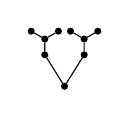
\begin{tikzpicture}[scale=0.2, every node/.style={circle, draw=black, fill=black, inner sep=0.75pt}]

        % Root node
        \node (root) at (0, -3) {};

        % Number of star graphs
        \def\nstars{2}

        % Leaves per star graph
        \def\leaves{3}

        % Radius for positioning leaves
        \def\radius{1}

        % Horizontal distance between star graphs
        \def\hstep{2.5}

        % Draw star graphs attached to the root node
        \foreach \i in {1,...,\nstars} {
          % Coordinates for the star's central node
          \node (c\i) at ({(\i-1)*\hstep - (\nstars-1)*\hstep/2}, 0) {};

          % Draw leaves around each star node
          \foreach \j in {1,...,\leaves} {
            \node (l\i\j) at ([shift={(270 - 360/\leaves + \j*360/\leaves: \radius)}] c\i) {};
            \draw (c\i) -- (l\i\j);
          }

          % Find the lowest leaf (typically the one at 270 degrees)
          \draw (root) -- (l\i1);
        }

      \end{tikzpicture}
      \caption*{$B(2, 4)$}
    \end{subfigure}
    \hspace*{1cm}
    \begin{subfigure}{0.1\textwidth}
      \centering
      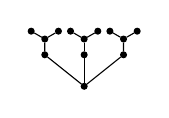
\begin{tikzpicture}[scale=0.2, every node/.style={circle, draw=black, fill=black, inner sep=0.75pt}]

        % Root node
        \node (root) at (0, -3) {};

        % Number of star graphs
        \def\nstars{3}

        % Leaves per star graph
        \def\leaves{3}

        % Radius for positioning leaves
        \def\radius{1}

        % Horizontal distance between star graphs
        \def\hstep{2.5}

        % Draw star graphs attached to the root node
        \foreach \i in {1,...,\nstars} {
          % Coordinates for the star's central node
          \node (c\i) at ({(\i-1)*\hstep - (\nstars-1)*\hstep/2}, 0) {};

          % Draw leaves around each star node
          \foreach \j in {1,...,\leaves} {
            \node (l\i\j) at ([shift={(270 - 360/\leaves + \j*360/\leaves: \radius)}] c\i) {};
            \draw (c\i) -- (l\i\j);
          }

          % Find the lowest leaf (typically the one at 270 degrees)
          \draw (root) -- (l\i1);
        }

      \end{tikzpicture}
      \caption*{$B(3, 4)$}
    \end{subfigure}
    \hspace*{1cm}
    \begin{subfigure}{0.15\textwidth}
      \centering
      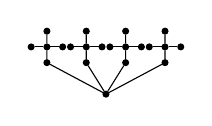
\begin{tikzpicture}[scale=0.2, every node/.style={circle, draw=black, fill=black, inner sep=0.75pt}]

        % Root node
        \node (root) at (0, -3) {};

        % Number of star graphs
        \def\nstars{4}

        % Leaves per star graph
        \def\leaves{4}

        % Radius for positioning leaves
        \def\radius{1}

        % Horizontal distance between star graphs
        \def\hstep{2.5}

        % Draw star graphs attached to the root node
        \foreach \i in {1,...,\nstars} {
          % Coordinates for the star's central node
          \node (c\i) at ({(\i-1)*\hstep - (\nstars-1)*\hstep/2}, 0) {};

          % Draw leaves around each star node
          \foreach \j in {1,...,\leaves} {
            \node (l\i\j) at ([shift={(270 - 360/\leaves + \j*360/\leaves: \radius)}] c\i) {};
            \draw (c\i) -- (l\i\j);
          }

          % Find the lowest leaf (typically the one at 270 degrees)
          \draw (root) -- (l\i1);
        }

      \end{tikzpicture}
      \caption*{$B(4, 5)$}
    \end{subfigure}

    \vspace*{0.5cm}

    \begin{subfigure}{0.15\textwidth}
      \centering
      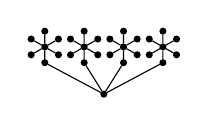
\begin{tikzpicture}[scale=0.2, every node/.style={circle, draw=black, fill=black, inner sep=0.75pt}]

        % Root node
        \node (root) at (0, -3) {};

        % Number of star graphs
        \def\nstars{4}

        % Leaves per star graph
        \def\leaves{6}

        % Radius for positioning leaves
        \def\radius{1}

        % Horizontal distance between star graphs
        \def\hstep{2.5}

        % Draw star graphs attached to the root node
        \foreach \i in {1,...,\nstars} {
          % Coordinates for the star's central node
          \node (c\i) at ({(\i-1)*\hstep - (\nstars-1)*\hstep/2}, 0) {};

          % Draw leaves around each star node
          \foreach \j in {1,...,\leaves} {
            \node (l\i\j) at ([shift={(270 - 360/\leaves + \j*360/\leaves: \radius)}] c\i) {};
            \draw (c\i) -- (l\i\j);
          }

          % Find the lowest leaf (typically the one at 270 degrees)
          \draw (root) -- (l\i1);
        }

      \end{tikzpicture}
      \caption*{$B(4, 7)$}
    \end{subfigure}
    \hspace*{1cm}
    \begin{subfigure}{0.2\textwidth}
      \centering
      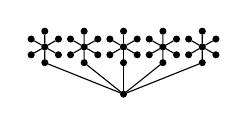
\begin{tikzpicture}[scale=0.2, every node/.style={circle, draw=black, fill=black, inner sep=0.75pt}]

        % Root node
        \node (root) at (0, -3) {};

        % Number of star graphs
        \def\nstars{5}

        % Leaves per star graph
        \def\leaves{6}

        % Radius for positioning leaves
        \def\radius{1}

        % Horizontal distance between star graphs
        \def\hstep{2.5}

        % Draw star graphs attached to the root node
        \foreach \i in {1,...,\nstars} {
          % Coordinates for the star's central node
          \node (c\i) at ({(\i-1)*\hstep - (\nstars-1)*\hstep/2}, 0) {};

          % Draw leaves around each star node
          \foreach \j in {1,...,\leaves} {
            \node (l\i\j) at ([shift={(270 - 360/\leaves + \j*360/\leaves: \radius)}] c\i) {};
            \draw (c\i) -- (l\i\j);
          }

          % Find the lowest leaf (typically the one at 270 degrees)
          \draw (root) -- (l\i1);
        }

      \end{tikzpicture}
      \caption*{$B(5, 7)$}
    \end{subfigure}

    \label{fig:banana-trees}
  \end{figure}
\end{frame}

\begin{frame}{Rooted Standard Form and isomorphic labelings}
  \begin{figure}[H]
    \centering
    \begin{adjustbox}{center}
      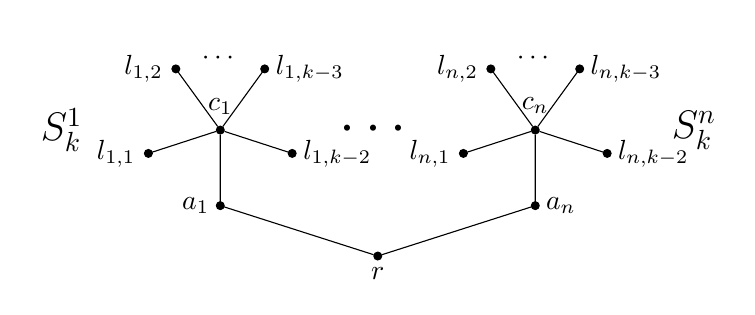
\begin{tikzpicture}[scale=0.8, every node/.style={circle, draw, fill=black, inner sep=1pt}]

        \node[label=below:{$r$}] (central) at (0, -2) {};

        \def\k{5} % Number of leaves in each star graph
        \def\leafradius{1.2} % Radius of the circular arrangement of leaves

        \node[label=above:{$c_1$}] (b1) at (-2.5, 0) {};
        \node[label=above:{$c_n$}] (b2) at (2.5, 0) {};

        \foreach \j in {1,...,\k} {
          \pgfmathsetmacro\leafangle{-90 - 360/\k * (\j-1)}

          \coordinate (l1\j) at ($(b1) + (\leafangle:\leafradius)$);
          \coordinate (l2\j) at ($(b2) + (\leafangle:\leafradius)$);
        }

        \node[label=left:{$a_1$}] at (l11) {};
        \node[label=left:{$l_{1,1}$}] at (l12) {};
        \node[label=left:{$l_{1,2}$}] at (l13) {};
        \node[label=right:{$l_{1,k-3}$}] at (l14) {};
        \node[label=right:{$l_{1,k-2}$}] at (l15) {};

        \draw (b1) -- (l11);
        \draw (b1) -- (l12);
        \draw (b1) -- (l13);
        \draw (b1) -- (l14);
        \draw (b1) -- (l15);

        \node[label=right:{$a_n$}] at (l21) {};
        \node[label=left:{$l_{n,1}$}] at (l22) {};
        \node[label=left:{$l_{n,2}$}] at (l23) {};
        \node[label=right:{$l_{n,k-3}$}] at (l24) {};
        \node[label=right:{$l_{n,k-2}$}] at (l25) {};

        \draw (b2) -- (l21);
        \draw (b2) -- (l22);
        \draw (b2) -- (l23);
        \draw (b2) -- (l24);
        \draw (b2) -- (l25);

        \foreach \j in {1,...,2} {
          \pgfmathsetmacro\dotangle{90}
          \node[draw=none, fill=none] at ($(b\j) + (\dotangle:0.95*\leafradius)$) {\textbf{$\cdots$}};
        }

        \node[draw=none, fill=none] at ($(b1) + (180:2.1*\leafradius)$) {\Large \textbf{$S^1_k$}};
        \node[draw=none, fill=none] at ($(b2) + (0:2.1*\leafradius)$) {\Large \textbf{$S^n_k$}};

        \draw (central) -- (l11);
        \draw (central) -- (l21);

        % Optional: add dots to indicate missing parts in the middle
        \node[draw=none,fill=none] at (0,0) {\huge \textbf{$\cdots$}};

      \end{tikzpicture}
    \end{adjustbox}

    \caption{Rooted standard form of a $B(n, k)$ tree}
    \label{fig:rsf-banana-tree}
  \end{figure}
  \vspace{-0.5em}
  We introduced notation for simpler representation of $\alpha$-labelings of $B(n, k)$ trees:
  \begin{itemize}
    \item The set of all leaves of the $i$-th star -- $\mathcal{L}_i = \{l_{i,j} \mid j \in [k-2] \}$
    \item The set of all non-central nodes of the $i$-th star -- $\mathcal{B}_i$ = $\{a_i\} \cup \mathcal{L}_i$
  \end{itemize}
  \begin{block}{Note}
    Swapping the labels of two leaves or two stars doesn't change the labeling.
  \end{block}
\end{frame}

\begin{frame}{Known results}
  \begin{block}{Theorem [G.~Sethuraman; J.~J.~Jesintha, 2009.]}
    All banana trees are graceful.
  \end{block}
  \begin{block}{Theorem}
    \begin{enumerate}
      \item All complete bipartite graphs $K_{m,n}$ are $\alpha$-labelable. ($B(n,1) \cong K_{1,n}$) [A.~Rosa, 1967.]
      \item The banana tree $B(n, k)$ is $\alpha$-labelable if $k > n$. [S.~Nikson; P.~S.~Ikhlas; A.~S.~Kiki, 2023.]
    \end{enumerate}
  \end{block}
\end{frame}

\section{Our results}

\begin{frame}{The set of labelings \( B(n, k) \)}
  \begin{block}{Definition [BG, Nakic, 202?]}
    Let $\mathcal{A}(n,k)$ be the set of all $\alpha$-labelings of the $B(n,k)$ tree and $\mathcal{A}_x(n,k)$ be the set of all $\alpha$-labelings of the $B(n,k)$ tree where $f(r) = x$. Let the set of principal $\alpha$-labelings $\mathcal{P}(n,k)$ be defined as $\mathcal{P}(n, k) = \bigcup\limits_{x = 1}^{\lfloor \frac{n}{2} \rfloor + 1} \mathcal{A}_x(n, k).$ Lastly, let the set of \textit{central} $\alpha$-labelings $\mathcal{C}(n,k)$ be defined as $\mathcal{C}(n, k) = \mathcal{A}_{\lfloor \frac{n}{2} \rfloor + 1}(n, k)$.
  \end{block}
  \begin{block}{Proposition [BG, Nakic, 202?]}
    Let $f$ be an $\alpha$-labeling of the $B(n,k)$ tree for any $n \in \mathbb{N}$ and $k \ge 2$. Then,
    $$
    f(r) \le \alpha \iff f(c_i) \le \alpha \quad \forall i \in [n]
    $$
  \end{block}
\end{frame}

\begin{frame}{Partitioning \( \mathcal{A}(n, k) \)}
  \begin{block}{Theorem [BG, Nakic, 202?]}
    For every $n, k \in \mathbb{N}$, we have
    $$
    \mathcal{A}(n, k) = \mathcal{P}(n, k) \cup \mathcal{P}^r(n, k) \cup \overline{\mathcal{P}}(n, k) \cup \overline{\mathcal{P}^r}(n, k),
    $$
    where $\mathcal{P}^r(n, k) = \{f^r : f \in \mathcal{P}(n, k)\}$, $\overline{\mathcal{P}}(n, k) = \{\overline{f} : f \in \mathcal{P}(n, k)\}$ and $\overline{\mathcal{P}^r}(n, k) = \{\overline{f^r} : f \in \mathcal{P}(n, k)\}$.
  \end{block}
  \begin{itemize}
    \item Reducing the set of possible $\alpha$-labelings by a factor of 4
    \item Reducing the complexity of the proofs
  \end{itemize}
\end{frame}

\begin{frame}{Classifying all the \(\alpha\)-labelings of all the \( B(n, 1) \) trees}
  \begin{block}{Theorem [BG, Nakic, 202?]}
    The $B(n, 1)$ tree is $\alpha$-labelable for all $n \in \mathbb{N}$. For $n = 1$ there exists a unique $\alpha$-labeling. For $n \geq 2$ there exist exactly 2 distinct $\alpha$-labelings.
  \end{block}

  \begin{figure}[H]
    \centering
    \begin{minipage}{0.4\textwidth}
      \centering
      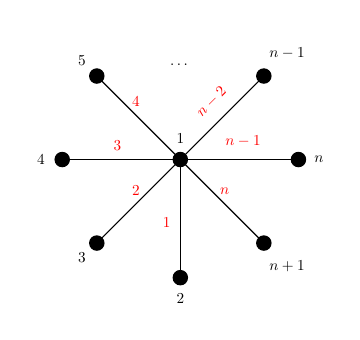
\begin{tikzpicture}[scale=0.75, every node/.style={circle, draw, fill=black, scale=0.55}, tight/.style={inner sep=0.02pt}]
        % Define the number of leaf vertices
        \def\n{7}
        % Define the radius for the leaf vertices
        \def\radius{2cm}

        % Draw the central vertex
        \node[circle, draw, fill=black, label=above:{$1$}] (C) at (0,0) {};

        % Draw the leaf vertices and connect them to the central vertex
        \foreach \i in {1,...,\n}
        {
          % Place each leaf vertex in a circular arrangement
          \coordinate (V\i) at ({135 + 360/(\n + 1) * (\i - 1)}:\radius) {};
          % Draw edge from central vertex to each leaf vertex
        }

        \node[circle, draw, fill=black, label=above left:{$5$}] at (V1) {};
        \node[circle, draw, fill=black, label=left:{$4$}] at (V2) {};
        \node[circle, draw, fill=black, label=below left:{$3$}] at (V3) {};
        \node[circle, draw, fill=black, label=below:{$2$}] at (V4) {};
        \node[circle, draw, fill=black, label=below right:{$n+1$}] at (V5) {};
        \node[circle, draw, fill=black, label=right:{$n$}] at (V6) {};
        \node[circle, draw, fill=black, label=above right:{$n-1$}] at (V7) {};

        \draw (C) -- (V1) node[midway, above, text=red, fill=none, draw=none] {$4$};
        \draw (C) -- (V2) node[midway, above, text=red, fill=none, draw=none] {$3$};
        \draw (C) -- (V3) node[midway, above, text=red, fill=none, draw=none] {$2$};
        \draw (C) -- (V4) node[midway, left, text=red, fill=none, draw=none] {$1$};
        \draw (C) -- (V5) node[midway, above, text=red, fill=none, draw=none] {$n$};
        \draw (C) -- (V6) node[tight, midway, above, text=red, fill=none, draw=none] {$n-1$};
        \draw (C) -- (V7) node[tight, midway, above, sloped, text=red, fill=none, draw=none] {$n-2$};

        \node[draw=none, fill=none] (dots) at (90:0.8*\radius) {\textbf{$\cdots$}};
      \end{tikzpicture}
      \caption*{$\alpha$-labeling $f_1$ with $\alpha = 1$} \label{fig:B(n,1)a}
    \end{minipage}
    \hspace{1cm}
    \begin{minipage}{0.4\textwidth}
      \centering
      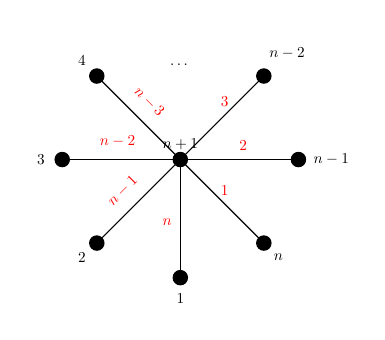
\begin{tikzpicture}[scale=0.75, every node/.style={circle, draw, fill=black, scale=0.55}, tight/.style={inner sep=0.02pt}]
        % Define the number of leaf vertices
        \def\n{7}
        % Define the radius for the leaf vertices
        \def\radius{2cm}

        % Draw the central vertex
        \node[circle, draw, fill=black] (C) at (0,0) {};
        \node[draw=none, fill=none, label={$n+1$}] at (0, -0.3) {};

        % Draw the leaf vertices and connect them to the central vertex
        \foreach \i in {1,...,\n}
        {
          % Place each leaf vertex in a circular arrangement
          \coordinate (V\i) at ({135 + 360/(\n + 1) * (\i - 1)}:\radius) {};
          % Draw edge from central vertex to each leaf vertex
        }

        \node[circle, draw, fill=black, label=above left:{$4$}] at (V1) {};
        \node[circle, draw, fill=black, label=left:{$3$}] at (V2) {};
        \node[circle, draw, fill=black, label=below left:{$2$}] at (V3) {};
        \node[circle, draw, fill=black, label=below:{$1$}] at (V4) {};
        \node[circle, draw, fill=black, label=below right:{$n$}] at (V5) {};
        \node[circle, draw, fill=black, label=right:{$n-1$}] at (V6) {};
        \node[circle, draw, fill=black, label=above right:{$n-2$}] at (V7) {};

        \draw (C) -- (V1) node[tight, midway, above, sloped, text=red, fill=none, draw=none] {$n-3$};
        \draw (C) -- (V2) node[tight, midway, above, text=red, fill=none, draw=none] {$n-2$};
        \draw (C) -- (V3) node[tight, midway, above, sloped, text=red, fill=none, draw=none] {$n-1$};
        \draw (C) -- (V4) node[midway, left, text=red, fill=none, draw=none] {$n$};
        \draw (C) -- (V5) node[midway, above, text=red, fill=none, draw=none] {$1$};
        \draw (C) -- (V6) node[midway, above, text=red, fill=none, draw=none] {$2$};
        \draw (C) -- (V7) node[midway, above, text=red, fill=none, draw=none] {$3$};

        \node[draw=none, fill=none] (dots) at (90:0.8*\radius) {\textbf{$\cdots$}};
      \end{tikzpicture}
      \caption*{$\alpha$-labeling $f_2$ with $\alpha = n$} \label{fig:B(n,1)b}
    \end{minipage}
    \caption{The two $\alpha$-labelings of $B(n, 1)$} \label{fig:B(n,1)}
  \end{figure}
\end{frame}

\begin{frame}{Classifying all the \(\alpha\)-labelings of all the \( B(1, k) \) trees}
  \begin{block}{Theorem [BG, Nakic, 202?]}
    The $B(1, 2)$ tree and the $B(1, 3)$ tree are have exactly 2 distinct $\alpha$-labelings.
  \end{block}

  \begin{figure}[H]
    \centering
    \begin{minipage}{0.4\textwidth}
      \centering
      \begin{minipage}{0.25\textwidth}
        \centering
        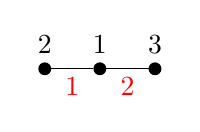
\begin{tikzpicture}[scale=0.35, every node/.style={circle, draw, fill=black, inner sep=1.5pt}]
          \node[label=above:{2}] (b1) at (-2, 0) {};

          \node[label=above:{1}] (central) at (0, 0) {};

          \node[label=above:{3}] (b2) at (2, 0) {};

          \draw (central) -- (b1) node[midway, below, text=red, fill=none, draw=none] {1};
          \draw (central) -- (b2) node[midway, below, text=red, fill=none, draw=none] {2};
        \end{tikzpicture}
      \end{minipage}
      \hspace{10mm}
      \begin{minipage}{0.25\textwidth}
        \centering
        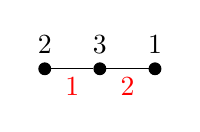
\begin{tikzpicture}[scale=0.35, every node/.style={circle, draw, fill=black, inner sep=1.5pt}]
          \node[label=above:{2}] (b1) at (-2, 0) {};

          \node[label=above:{3}] (central) at (0, 0) {};

          \node[label=above:{1}] (b2) at (2, 0) {};

          \draw (central) -- (b1) node[midway, below, text=red, fill=none, draw=none] {1};
          \draw (central) -- (b2) node[midway, below, text=red, fill=none, draw=none] {2};
        \end{tikzpicture}
      \end{minipage}
      \caption*{The $\alpha$-labelings of $B(1, 2)$}
    \end{minipage}
    \begin{minipage}{0.5\textwidth}
      \centering
      \begin{minipage}{0.25\textwidth}
        \centering
        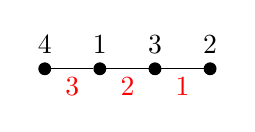
\begin{tikzpicture}[scale=0.35, every node/.style={circle, draw, fill=black, inner sep=1.5pt}]
          \node[label=above:{4}] (b1) at (-2, 0) {};

          \node[label=above:{1}] (central) at (0, 0) {};

          \node[label=above:{3}] (b2) at (2, 0) {};

          \node[label=above:{2}] (l11) at (4, 0) {};

          \draw (central) -- (b1) node[midway, below, text=red, fill=none, draw=none] {3};
          \draw (central) -- (b2) node[midway, below, text=red, fill=none, draw=none] {2};
          \draw (b2) -- (l11) node[midway, below, text=red, fill=none, draw=none] {1};
        \end{tikzpicture}
      \end{minipage}
      \hspace{12mm}
      \begin{minipage}{0.25\textwidth}
        \centering
        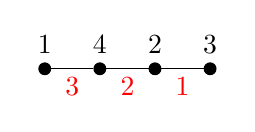
\begin{tikzpicture}[scale=0.35, every node/.style={circle, draw, fill=black, inner sep=1.5pt}]
          \node[label=above:{1}] (b1) at (-2, 0) {};

          \node[label=above:{4}] (central) at (0, 0) {};

          \node[label=above:{2}] (b2) at (2, 0) {};

          \node[label=above:{3}] (l11) at (4, 0) {};

          \draw (central) -- (b1) node[midway, below, text=red, fill=none, draw=none] {3};
          \draw (central) -- (b2) node[midway, below, text=red, fill=none, draw=none] {2};
          \draw (b2) -- (l11) node[midway, below, text=red, fill=none, draw=none] {1};
        \end{tikzpicture}
      \end{minipage}
      \caption*{The $\alpha$-labelings of $B(1, 3)$}
    \end{minipage}
  \end{figure}

  \begin{block}{Theorem [BG, Nakic, 202?]}
    The $B(1, k)$ tree is $\alpha$-labelable for $k \geq 4$ and has exactly 4 distinct $\alpha$-labelings.
  \end{block}
\end{frame}

\begin{frame}{Classifying all the \(\alpha\)-labelings of all the \( B(1, k) \) trees}
  \begin{figure}[H]
    \centering
    \begin{minipage}{0.4\textwidth}
      \centering
      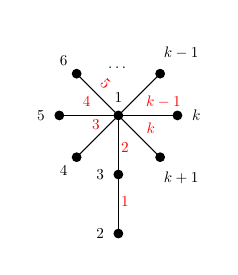
\begin{tikzpicture}[scale=0.5, every node/.style={circle, draw, fill=black, scale=0.55}, tight/.style={inner sep=0.02pt}]
        % Define the number of leaf vertices
        \def\n{7}
        % Define the radius for the leaf vertices
        \def\radius{1.5cm}

        % Draw the central vertex
        \node[circle, draw, fill=black, inner sep=2pt, label=above:1] (c) at (0,0) {};
        \node[circle, draw, fill=black, inner sep=2pt, label=left:2] (r) at (0,-3) {};

        % Draw the leaf vertices and connect them to the central vertex
        \foreach \i in {1,...,\n}
        {
          % Place each leaf vertex in a circular arrangement
          \coordinate (V\i) at ({135 + 360/(\n + 1) * (\i - 1)}:\radius) {};
          % Draw edge from central vertex to each leaf vertex
        }

        \node[circle, draw, fill=black, inner sep=2pt, label=above left:6] at (V1) {};
        \node[circle, draw, fill=black, inner sep=2pt, label=left:5] at (V2) {};
        \node[circle, draw, fill=black, inner sep=2pt, label=below left:4] at (V3) {};
        \node[circle, draw, fill=black, inner sep=2pt, label=left:3] at (V4) {};
        \node[circle, draw, fill=black, inner sep=2pt, label=below right:{$k+1$}] at (V5) {};
        \node[circle, draw, fill=black, inner sep=2pt, label=right:{$k$}] at (V6) {};
        \node[circle, draw, fill=black, inner sep=2pt, label=above right:{$k-1$}] at (V7) {};

        \draw (c) -- (V1) node[midway, above, sloped, text=red, fill=none, draw=none] {5};
        \draw (c) -- (V2) node[midway, above,  text=red, fill=none, draw=none] {4};
        \draw (c) -- (V3) node[midway, above, text=red, fill=none, draw=none] {3};
        \draw (c) -- (V4) node[tight, midway, above, text=red, right, fill=none, draw=none] {2};
        \draw (c) -- (V5) node[midway, above right, text=red, fill=none, draw=none] {$k$};
        \draw (c) -- (V6) node[tight, midway, above right, text=red, fill=none, draw=none] {$k-1$};
        \draw (c) -- (V7);

        \draw (V4) -- (r) node[tight, midway, right, text=red, fill=none, draw=none] {1};

        \node[draw=none, fill=none] (dots) at (90:0.8*\radius) {\textbf{$\cdots$}};
      \end{tikzpicture}

      \caption*{$\alpha$-labeling $f_1$ with $\alpha_1 = 2$} \label{fig:B(1,k)a}
    \end{minipage}
    \hspace*{1cm}
    \begin{minipage}{0.4\textwidth}
      \centering
      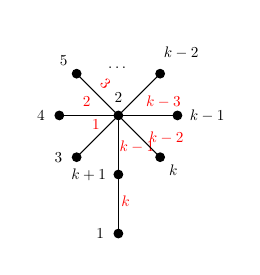
\begin{tikzpicture}[scale=0.5, every node/.style={circle, draw, fill=black, scale=0.55}, tight/.style={inner sep=0.02pt}]
        % Define the number of leaf vertices
        \def\n{7}
        % Define the radius for the leaf vertices
        \def\radius{1.5cm}

        % Draw the central vertex
        \node[circle, draw, fill=black, inner sep=2pt, label=above:2] (c) at (0,0) {};
        \node[circle, draw, fill=black, inner sep=2pt, label=left:1] (r) at (0,-3) {};

        % Draw the leaf vertices and connect them to the central vertex
        \foreach \i in {1,...,\n}
        {
          % Place each leaf vertex in a circular arrangement
          \coordinate (V\i) at ({135 + 360/(\n + 1) * (\i - 1)}:\radius) {};
          % Draw edge from central vertex to each leaf vertex
        }

        \node[circle, draw, fill=black, inner sep=2pt, label=above left:5] at (V1) {};
        \node[circle, draw, fill=black, inner sep=2pt, label=left:4] at (V2) {};
        \node[circle, draw, fill=black, inner sep=2pt, label=left:3] at (V3) {};
        \node[circle, draw, fill=black, inner sep=2pt, label=left:{$k+1$}] at (V4) {};
        \node[circle, draw, fill=black, inner sep=2pt, label=below right:{$k$}] at (V5) {};
        \node[circle, draw, fill=black, inner sep=2pt, label=right:{$k-1$}] at (V6) {};
        \node[circle, draw, fill=black, inner sep=2pt, label=above right:{$k-2$}] at (V7) {};

        \draw (c) -- (V1) node[midway, above, sloped, text=red, fill=none, draw=none] {3};
        \draw (c) -- (V2) node[midway, above, text=red, fill=none, draw=none] {2};
        \draw (c) -- (V3) node[midway, above, text=red, fill=none, draw=none] {1};
        \draw (c) -- (V4) node[tight, midway, right, text=red, fill=none, draw=none] {$k-1$};
        \draw (c) -- (V5) node[midway, right, text=red, fill=none, draw=none] {$k-2$};
        \draw (c) -- (V6) node[tight, midway, above right, text=red, fill=none, draw=none] {$k-3$};
        \draw (c) -- (V7);

        \draw (V4) -- (r) node[tight, midway, right, text=red, fill=none, draw=none] {$k$};

        \node[draw=none, fill=none] (dots) at (90:0.8*\radius) {\textbf{$\cdots$}};
      \end{tikzpicture}

      \caption*{$\alpha$-labeling $f_2$ with $\alpha_2 = 2$} \label{fig:B(1,k)b}
    \end{minipage}
    \begin{minipage}{0.4\textwidth}
      \centering
      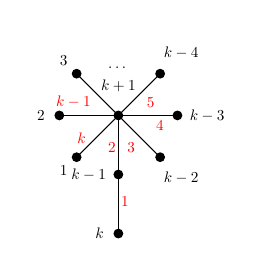
\begin{tikzpicture}[scale=0.5, every node/.style={circle, draw, fill=black, scale=0.55}, tight/.style={inner sep=0.02pt}]
        % Define the number of leaf vertices
        \def\n{7}
        % Define the radius for the leaf vertices
        \def\radius{1.5cm}

        % Draw the central vertex
        \node[circle, draw, fill=black, inner sep=2pt, label=above:{$k+1$}] (c) at (0,0) {};
        \node[circle, draw, fill=black, inner sep=2pt, label=left:{$k$}] (r) at (0,-3) {};

        % Draw the leaf vertices and connect them to the central vertex
        \foreach \i in {1,...,\n}
        {
          % Place each leaf vertex in a circular arrangement
          \coordinate (V\i) at ({135 + 360/(\n + 1) * (\i - 1)}:\radius) {};
          % Draw edge from central vertex to each leaf vertex
        }

        \node[circle, draw, fill=black, inner sep=2pt, label=above left:3] at (V1) {};
        \node[circle, draw, fill=black, inner sep=2pt, label=left:2] at (V2) {};
        \node[circle, draw, fill=black, inner sep=2pt, label=below left:1] at (V3) {};
        \node[circle, draw, fill=black, inner sep=2pt, label=left:{$k-1$}] at (V4) {};
        \node[circle, draw, fill=black, inner sep=2pt, label=below right:{$k-2$}] at (V5) {};
        \node[circle, draw, fill=black, inner sep=2pt, label=right:{$k-3$}] at (V6) {};
        \node[circle, draw, fill=black, inner sep=2pt, label=above right:{$k-4$}] at (V7) {};

        \draw (c) -- (V1);
        \draw (c) -- (V2) node[tight, midway, above left, text=red, fill=none, draw=none] {$k-1$};
        \draw (c) -- (V3) node[midway, left, text=red, fill=none, draw=none] {$k$};
        \draw (c) -- (V4) node[tight, midway, left, text=red, fill=none, draw=none] {2};
        \draw (c) -- (V5) node[midway, below left, text=red, fill=none, draw=none] {3};
        \draw (c) -- (V6) node[midway, below right, text=red, fill=none, draw=none] {4};
        \draw (c) -- (V7) node[midway, below right, text=red, fill=none, draw=none] {5};

        \draw (V4) -- (r) node[tight, midway, right, text=red, fill=none, draw=none] {1};

        \node[draw=none, fill=none] (dots) at (90:0.8*\radius) {\textbf{$\cdots$}};
      \end{tikzpicture}
      \caption*{$\alpha$-labeling $f_3$ with $\alpha_3 = k - 1$} \label{fig:B(1,k)c}
    \end{minipage}
    \hspace*{1cm}
    \begin{minipage}{0.4\textwidth}
      \centering
      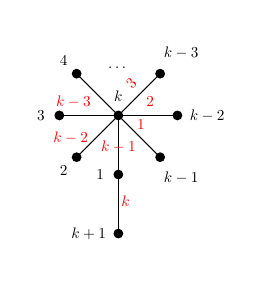
\begin{tikzpicture}[scale=0.5, every node/.style={circle, draw, fill=black, scale=0.55}, tight/.style={inner sep=0.02pt}]
        % Define the number of leaf vertices
        \def\n{7}
        % Define the radius for the leaf vertices
        \def\radius{1.5cm}

        % Draw the central vertex
        \node[circle, draw, fill=black, inner sep=2pt, label=above:{$k$}] (c) at (0,0) {};
        \node[circle, draw, fill=black, inner sep=2pt, label=left:{$k+1$}] (r) at (0,-3) {};

        % Draw the leaf vertices and connect them to the central vertex
        \foreach \i in {1,...,\n}
        {
          % Place each leaf vertex in a circular arrangement
          \coordinate (V\i) at ({135 + 360/(\n + 1) * (\i - 1)}:\radius) {};
          % Draw edge from central vertex to each leaf vertex
        }

        \node[circle, draw, fill=black, inner sep=2pt, label=above left:4] at (V1) {};
        \node[circle, draw, fill=black, inner sep=2pt, label=left:3] at (V2) {};
        \node[circle, draw, fill=black, inner sep=2pt, label=below left:2] at (V3) {};
        \node[circle, draw, fill=black, inner sep=2pt, label=left:{1}] at (V4) {};
        \node[circle, draw, fill=black, inner sep=2pt, label=below right:{$k-1$}] at (V5) {};
        \node[circle, draw, fill=black, inner sep=2pt, label=right:{$k-2$}] at (V6) {};
        \node[circle, draw, fill=black, inner sep=2pt, label=above right:{$k-3$}] at (V7) {};

        \draw (c) -- (V1);
        \draw (c) -- (V2) node[tight, midway, above left, text=red, fill=none, draw=none,] {$k-3$};
        \draw (c) -- (V3) node[midway, left, text=red, fill=none, draw=none] {$k-2$};
        \draw (c) -- (V4) node[tight, midway, text=red, fill=none, draw=none] {$k-1$};
        \draw (c) -- (V5) node[midway, above, text=red, fill=none, draw=none] {1};
        \draw (c) -- (V6) node[midway, above, text=red, fill=none, draw=none] {2};
        \draw (c) -- (V7) node[midway, above, sloped, text=red, fill=none, draw=none] {3};

        \draw (V4) -- (r) node[tight, midway, right, text=red, fill=none, draw=none] {$k$};

        \node[draw=none, fill=none] (dots) at (90:0.8*\radius) {\textbf{$\cdots$}};
      \end{tikzpicture}

      \caption*{$\alpha$-labeling $f_4$ with $\alpha_4 = k - 1$} \label{fig:B(1,k)d}
    \end{minipage}
    \caption{Four possible $\alpha$-labelings of $B(1, k)$} \label{fig:B(1,k)}
  \end{figure}
\end{frame}

\begin{frame}{Classifying all the \(\alpha\)-labelings of all the \( B(2, k) \) trees}
  \begin{block}{Theorem [BG, Nakic, 202?]}
    \vbox{\parindent=0pt
      \setlength\abovedisplayskip{0pt}
      \setlength\abovedisplayshortskip{0pt}
      \setlength\belowdisplayskip{0pt}
      \setlength\belowdisplayshortskip{0pt}
      $\mathcal{A}_1(2, 2) = \emptyset$ and for every $k \ge 3$, we have $\mathcal{A}_1(2, k) = \{f\}$, where
      \vspace{-0.8em}
      {\small
        $$
        \begin{array}{lcl}
          f(r) & = & 1 \\
          f(c_i) & = & i + 1 \\
          f(a_i) & = & (3 - i)k + 1 \\
          \mathcal{F}(\mathcal{L}_1) & = & \{k + 3, k + 4, \dots, 2k\}\\
          \mathcal{F}(\mathcal{L}_2) & = & \{4, 5, \dots, k-1, k, k+2\}\\
        \end{array}
        $$
      }
    }
    \vspace{-0.8em}
  \end{block}

  \vspace*{-0.5cm}

  \begin{figure}
    \centering
    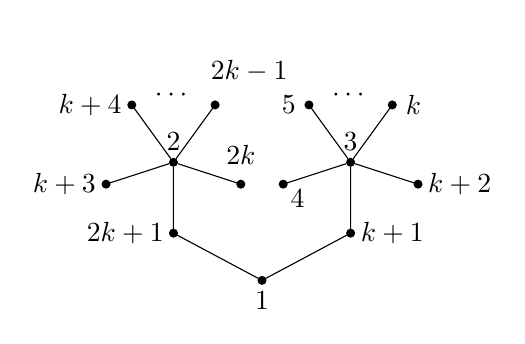
\begin{tikzpicture}[scale=0.75, every node/.style={circle, draw, fill=black, inner sep=1pt}]

      \node[label=below:{$1$}] (central) at (0, -2) {};

      \def\k{5} % Number of leaves in each star graph
      \def\leafradius{1.2} % Radius of the circular arrangement of leaves

      \node[label=above:{$2$}] (b1) at (-1.5, 0) {};
      \node[label=above:{$3$}] (b2) at (1.5, 0) {};

      \foreach \j in {1,...,\k} {
        \pgfmathsetmacro\leafangle{-90 - 360/\k * (\j-1)}

        \coordinate (l1\j) at ($(b1) + (\leafangle:\leafradius)$);
        \coordinate (l2\j) at ($(b2) + (\leafangle:\leafradius)$);
      }

      \node[label=left:{$2k + 1$}] at (l11) {};
      \node[label=left:{$k + 3$}] at (l12) {};
      \node[label=left:{$k + 4$}] at (l13) {};
      \node[label=above right:{$2k - 1$}] at (l14) {};
      \node at (l15) {};
      \node[draw=none, fill=none] at ([yshift=5mm]l15) {$2k$};

      \draw (b1) -- (l11);
      \draw (b1) -- (l12);
      \draw (b1) -- (l13);
      \draw (b1) -- (l14);
      \draw (b1) -- (l15);

      \node[label=right:{$k + 1$}] at (l21) {};
      \node[label=below right:{$4$}] at (l22) {};
      \node[label=left:{$5$}] at (l23) {};
      \node[label=right:{$k$}] at (l24) {};
      \node[label=right:{$k + 2$}] at (l25) {};

      \draw (b2) -- (l21);
      \draw (b2) -- (l22);
      \draw (b2) -- (l23);
      \draw (b2) -- (l24);
      \draw (b2) -- (l25);

      \foreach \j in {1,...,2} {
        \pgfmathsetmacro\dotangle{90}
        \node[draw=none, fill=none] at ($(b\j) + (\dotangle:0.95*\leafradius)$) {\textbf{$\cdots$}};
      }

      \draw (central) -- (l11);
      \draw (central) -- (l21);
    \end{tikzpicture}
    \caption*{$\alpha$-labeling $f \in \mathcal{A}_1(2, k)$ with $\alpha = 3$}
  \end{figure}
\end{frame}

\begin{frame}{Classifying all the \(\alpha\)-labelings of all the \( B(2, k) \) trees}
  \begin{block}{Theorem [BG, Nakic, 202?]}
    \vbox{\parindent=0pt
      \setlength\abovedisplayskip{0pt}
      \setlength\abovedisplayshortskip{0pt}
      \setlength\belowdisplayskip{0pt}
      \setlength\belowdisplayshortskip{0pt}
      For every $k \ge 2$, we have $\mathcal{A}_2(2, k) = \{f_y \mid k + 3 \le y \le 2k + 1\}$, where
      \vspace{-0.8em}
      {\small
        $$
        \begin{array}{lcl}
          f_y(r) & = & 2, \quad f_y(c_1) = 1, \quad f_y(c_2) = 3 \\
          f_y(a_1) & = & y \\
          f_y(a_2) & = & 2k + 5 - y \\
          \mathcal{F}_y(\mathcal{L}_1) & = & \{y + 1, y + 2, \dots, 2k + 1\} \cup \{y - 2i \mid 1 \le i \le y - k - 3\}\\
          \mathcal{F}_y(\mathcal{L}_2) & = & \left( \{4, 5, \dots, 2k + 4 - y\} \cup \{2k + 5 - y + 2i \mid 1 \le i \le y - k - 3\} \right)\\
        \end{array}
        $$
      }
      \vspace{-0.8em}
    }
  \end{block}

  \vspace*{-0.75cm}

  \begin{figure}[H]
    \centering
    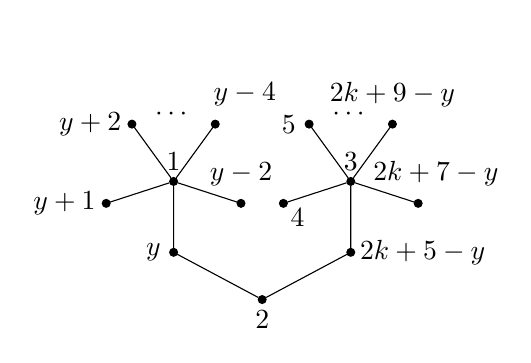
\begin{tikzpicture}[scale=0.75, every node/.style={circle, draw, fill=black, inner sep=1pt}]

      \node[label=below:{$2$}] (central) at (0, -2) {};

      \def\k{5} % Number of leaves in each star graph
      \def\leafradius{1.2} % Radius of the circular arrangement of leaves

      \node[label=above:{$1$}] (b1) at (-1.5, 0) {};
      \node[label=above:{$3$}] (b2) at (1.5, 0) {};

      \foreach \j in {1,...,\k} {
        \pgfmathsetmacro\leafangle{-90 - 360/\k * (\j-1)}

        \coordinate (l1\j) at ($(b1) + (\leafangle:\leafradius)$);
        \coordinate (l2\j) at ($(b2) + (\leafangle:\leafradius)$);
      }

      \node[label=left:{$y$}] at (l11) {};
      \node[label=left:{$y + 1$}] at (l12) {};
      \node[label=left:{$y + 2$}] at (l13) {};
      \node[label=above right:{$y - 4$}] at (l14) {};
      \node at (l15) {};
      \node[draw=none, fill=none] at ([yshift=5mm]l15) {$y - 2$};

      \draw (b1) -- (l11);
      \draw (b1) -- (l12);
      \draw (b1) -- (l13);
      \draw (b1) -- (l14);
      \draw (b1) -- (l15);

      \node[label=right:{$2k + 5 - y$}] at (l21) {};
      \node[label=below right:{$4$}] at (l22) {};
      \node[label=left:{$5$}] at (l23) {};
      \node at (l24) {};
      \node at (l25) {};
      \node[draw=none, fill=none] at ([yshift=5mm]l24) {$2k + 9 - y$};
      \node[draw=none, fill=none] at ([yshift=5mm, xshift=3mm]l25) {$2k + 7 - y$};

      \draw (b2) -- (l21);
      \draw (b2) -- (l22);
      \draw (b2) -- (l23);
      \draw (b2) -- (l24);
      \draw (b2) -- (l25);

      \foreach \j in {1,...,2} {
        \pgfmathsetmacro\dotangle{90}
        \node[draw=none, fill=none] at ($(b\j) + (\dotangle:0.95*\leafradius)$) {\textbf{$\cdots$}};
      }

      \draw (central) -- (l11);
      \draw (central) -- (l21);
    \end{tikzpicture}
    \caption*{$\alpha$-labeling $f_y \in \mathcal{A}_2(2, k)$ with $\alpha = 3$}
  \end{figure}
\end{frame}

\begin{frame}{A sketch of the proof for \( B(n, k) \) for \( k > n \)}
  \begin{block}{Theorem [BG, Nakic, 202?]}
    The $B(n, k)$ tree is $\alpha$-labelable for all $n \geq 3$ and $k > n$.
  \end{block}

  Labeling which proves the theorem:

  \vspace{-1cm}

  \begin{figure}[H]
    \centering
    \begin{adjustbox}{max width=1.1\textwidth,center}
      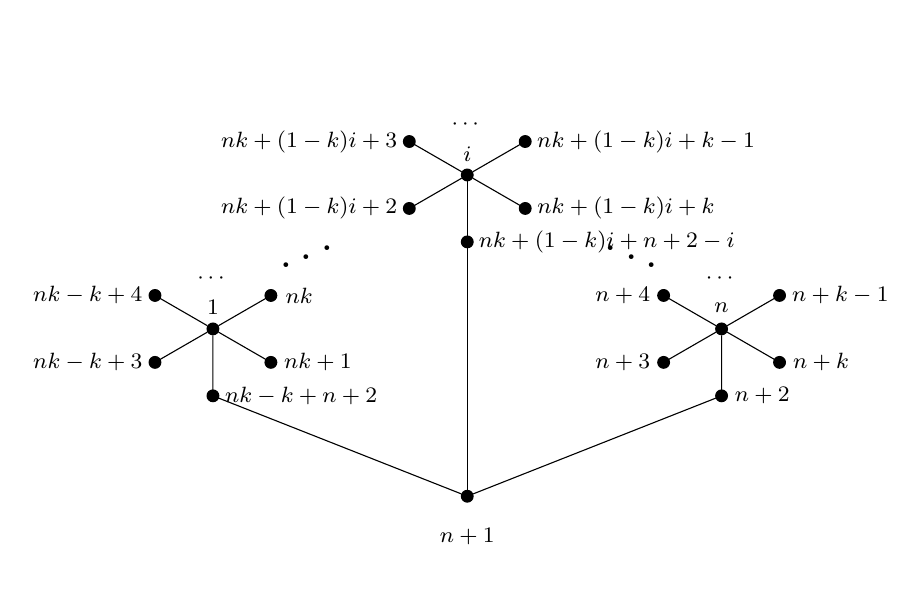
\begin{tikzpicture}[scale=0.85, every node/.style={circle, draw, fill=black, inner sep=1.5pt, font=\footnotesize}]

        \node[label=below:{$ n + 1$}] (central) at (0, -2.5) {};

        \def\k{6} % Number of leaves in each star graph
        \def\leafradius{1} % Radius of the circular arrangement of leaves

        \node[label=above:{$1$}] (b1) at (-3.8, 0) {};
        \node[label=above:{$i$}] (b2) at (0, 2.3) {};
        \node[label=above:{$n$}] (b3) at (3.8, 0) {};

        \foreach \j in {1,...,\k} {
          \pgfmathsetmacro\leafangle{-90 - 360/\k * (\j-1)}

          \coordinate (l1\j) at ($(b1) + (\leafangle:\leafradius)$);
          \coordinate (l2\j) at ($(b2) + (\leafangle:\leafradius)$);
          \coordinate (l3\j) at ($(b3) + (\leafangle:\leafradius)$);
        }

        \node[label=right:{$nk -k + n + 2$}] at (l11) {};
        \node[label=left:{$nk - k + 3$}] at (l12) {};
        \node[label=left:{$nk - k + 4$}] at (l13) {};
        \node[label=right:{$nk$}] at (l15) {};
        \node[label=right:{$nk + 1$}] at (l16) {};

        \draw (b1) -- (l11);
        \draw (b1) -- (l12);
        \draw (b1) -- (l13);
        \draw (b1) -- (l15);
        \draw (b1) -- (l16);

        \node[label=right:{$nk + (1-k)i + n + 2 -i $}] at (l21) {};
        \node[label=left:{$nk + (1-k)i +2$}] at (l22) {};
        \node[label=left:{$nk + (1-k)i + 3$}] at (l23) {};
        \node[label=right:{$nk + (1-k)i + k - 1$}] at (l25) {};
        \node[label=right:{$nk + (1-k)i + k$}] at (l26) {};

        \draw (b2) -- (l21);
        \draw (b2) -- (l22);
        \draw (b2) -- (l23);
        \draw (b2) -- (l25);
        \draw (b2) -- (l26);

        \node[label=right:{$n + 2$}] at (l31) {};
        \node[label=left:{$n + 3$}] at (l32) {};
        \node[label=left:{$n + 4$}] at (l33) {};
        \node[label=right:{$n + k - 1$}] at (l35) {};
        \node[label=right:{$n + k$}] at (l36) {};

        \draw (b3) -- (l31);
        \draw (b3) -- (l32);
        \draw (b3) -- (l33);
        \draw (b3) -- (l35);
        \draw (b3) -- (l36);

        \foreach \j in {1,...,3} {
          \pgfmathsetmacro\dotangle{90}
          \node[draw=none, fill=none] at ($(b\j) + (\dotangle:0.75*\leafradius)$) {\textbf{$\cdots$}};
        }

        \draw (central) -- (l11);
        \draw (central) -- (l21);
        \draw (central) -- (l31);

        \node[draw=none,fill=none] at (-2.4,1.2) {\huge{\reflectbox{$\ddots$}}};
        \node[draw=none,fill=none] at (2.45,1.2) {\huge{$\ddots$}};

      \end{tikzpicture}
    \end{adjustbox}
    \label{fig:B(n,k)}
  \end{figure}
\end{frame}

\begin{frame}{A sketch of the proof for \( B(n, k) \) for \( \frac{n}{2} + 1 \le k \le n\)}
  \begin{block}{Theorem [BG, Nakic, 202?]}
    The $B(n, k)$ tree is $\alpha$-labelable for all $n \in \mathbb{N}$ and $\frac{n}{2} + 1 \leq k \leq n + 1$.
  \end{block}

  Labeling which proves the theorem:

  \begin{align*}\label{eq:Tm5}
    \begin{split}
      f(r) &= n + 2 - k \\
      f(c_i) &=
      \begin{cases}
        n + 2 - i, & i < k \\
        n + 1 - i, & i \geq k
      \end{cases} \\
      f(a_i) &=
      \begin{cases}
        n + 2 -k + ki, & i < k \\
        n + 3 - 2k + ki, & i \geq k
      \end{cases} \\
      \mathcal{F}(\mathcal{L}_i) &= \{n + 3 -k + (k - 1) i, \dots, n + 1 + (k - 1) i\} \setminus \{f(a_i)\}
    \end{split}
  \end{align*}
\end{frame}

\begin{frame}{A sketch of the proof for \( B(n, k) \) for \( \frac{n}{2} + 1 \le k \le n\)}
  \begin{figure}[H]
    \centering
    \begin{adjustbox}{max width=1.2\textwidth,center}
      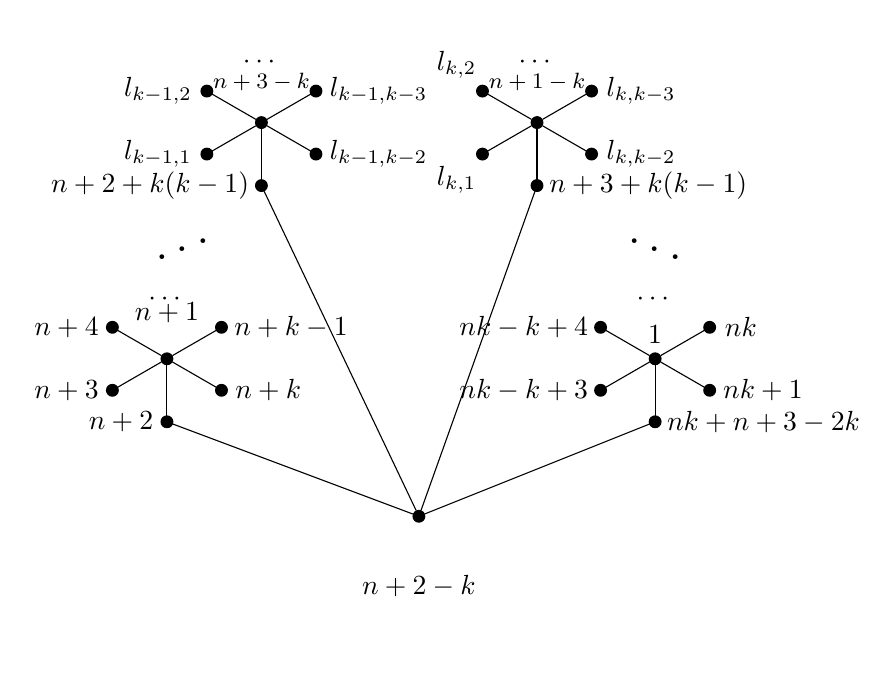
\begin{tikzpicture}[scale=1, every node/.style={circle, draw, fill=black, inner sep=1.5pt}]

        \node[label=below:{$n + 2 - k$}] (central) at (0, -2) {};

        \def\k{6} % Number of leaves in each star graph
        \def\leafradius{0.8} % Radius of the circular arrangement of leaves

        \node[label=above:{$n + 1$}] (b1) at (-3.2, 0) {};
        \node[label={[label distance = -0.25cm]above:{\footnotesize $n + 3 - k$}}] (b2) at (-2, 3) {};
        \node[label={[label distance = -0.25cm]above:{\footnotesize $n + 1 - k$}}] (b4) at (1.5, 3) {};
        \node[label=above:{$1$}] (b3) at (3, 0) {};

        \foreach \j in {1,...,\k} {
          \pgfmathsetmacro\leafangle{-90 - 360/\k * (\j-1)}

          \coordinate (l1\j) at ($(b1) + (\leafangle:\leafradius)$);
          \coordinate (l2\j) at ($(b2) + (\leafangle:\leafradius)$);
          \coordinate (l3\j) at ($(b3) + (\leafangle:\leafradius)$);
          \coordinate (l4\j) at ($(b4) + (\leafangle:\leafradius)$);
        }

        \node[label=left:{$n + 2$}] at (l11) {};
        \node[label=left:{$n + 3$}] at (l12) {};
        \node[label=left:{$n + 4$}] at (l13) {};
        \node[label=right:{$n + k - 1$}] at (l15) {};
        \node[label=right:{$n + k$}] at (l16) {};

        \draw (b1) -- (l11);
        \draw (b1) -- (l12);
        \draw (b1) -- (l13);
        \draw (b1) -- (l15);
        \draw (b1) -- (l16);

        \node[label=left:{$n + 2 + k(k-1)$}] at (l21) {};
        \node[label=left:{$l_{k-1,1}$}] at (l22) {};
        \node[label=left:{$l_{k-1,2}$}] at (l23) {};
        \node[label=right:{$l_{k-1,k-3}$}] at (l25) {};
        \node[label=right:{$l_{k-1,k-2}$}] at (l26) {};

        \draw (b2) -- (l21);
        \draw (b2) -- (l22);
        \draw (b2) -- (l23);
        \draw (b2) -- (l25);
        \draw (b2) -- (l26);

        \node[label=right:{$nk + n + 3 - 2k$}] at (l31) {};
        \node[label=left:{$nk - k + 3$}] at (l32) {};
        \node[label=left:{$nk - k + 4$}] at (l33) {};
        \node[label=right:{$nk$}] at (l35) {};
        \node[label=right:{$nk + 1$}] at (l36) {};

        \draw (b3) -- (l31);
        \draw (b3) -- (l32);
        \draw (b3) -- (l33);
        \draw (b3) -- (l35);
        \draw (b3) -- (l36);

        \node[label=right:{$n + 3 + k(k-1)$}] at (l41) {};
        \node[label=below left:{$l_{k,1}$}] at (l42) {};
        \node[label=above left:{$l_{k,2}$}] at (l43) {};
        \node[label=right:{$l_{k,k-3}$}] at (l45) {};
        \node[label=right:{$l_{k,k-2}$}] at (l46) {};

        \draw (b4) -- (l41);
        \draw (b4) -- (l42);
        \draw (b4) -- (l43);
        \draw (b4) -- (l45);
        \draw (b4) -- (l46);

        \foreach \j in {1,...,4} {
          \pgfmathsetmacro\dotangle{90}
          \node[draw=none, fill=none] at ($(b\j) + (\dotangle:0.95*\leafradius)$) {\textbf{$\cdots$}};
        }

        \draw (central) -- (l11);
        \draw (central) -- (l21);
        \draw (central) -- (l31);
        \draw (central) -- (l41);

        % Optional: add dots to indicate missing parts in the middle
        \node[draw=none,fill=none] at (-3,1.5) {\huge{\reflectbox{$\ddots$}}};
        \node[draw=none,fill=none] at (3,1.5) {\huge{$\ddots$}};

      \end{tikzpicture}
    \end{adjustbox}
    \label{fig:B(n,k)2}
  \end{figure}
\end{frame}

\section{Conclusion}

\begin{frame}{$\alpha$-labelability of $B(n, k)$ trees}
  \begin{block}{Corollary [BG, Nakic, 202?]}
    The $B(n, k)$ tree is $\alpha$-labelable if and only if either $k \geq \frac{n}{2} + 1$ or $k = 1$.
  \end{block}
  \begin{figure}[H]
    \centering
    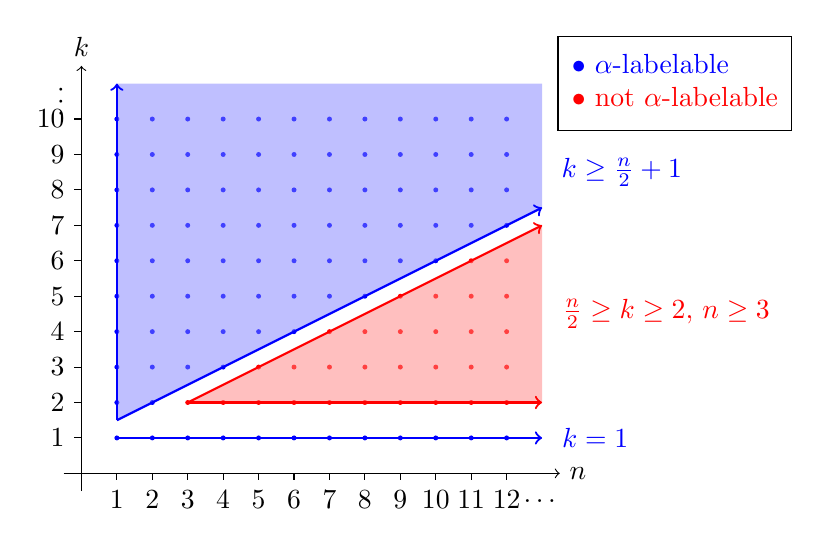
\begin{tikzpicture}[scale=0.45]
      % Draw grid points for integer lattice
      \foreach \y in {2,...,10} {
        \pgfmathparse{min(12, 2*\y-2)}
        \let\xmax\pgfmathresult
        \foreach \x in {1,...,\xmax} {
          \fill[blue] (\x,\y) circle (2pt);
        }
      }

      % Highlight the region k >= n/2 + 1
      \fill[blue!50, opacity=0.5] (1,1.5) -- (13,7.5) -- (13,11) -- (1,11) -- cycle;
      \draw[blue, thick, ->] (1,1.5) -- (13,7.5);
      \draw[blue, thick, ->] (1,1.5) -- (1,11);

      \foreach \x in {1,...,12} {
        \fill[blue] (\x,1) circle (2pt);
      }

      % Highlight the line k = 1
      \draw[blue, thick, ->] (1,1) -- (13,1);

      \foreach \x in {3,...,12} {
        \pgfmathsetmacro{\ymax}{(\x+1)/2}
        \foreach \y in {2,...,\ymax} {
          \fill[red] (\x,\y) circle (2pt);
        }
      }

      % HIghlight the unknown region
      \fill[red!50, opacity=0.5] (3,2) -- (13,2) -- (13,7) -- cycle;
      \draw[red, thick, ->] (3,2) -- (13,2);
      \draw[red, thick, ->] (3,2) -- (13,7);

      % Draw axes
      \draw[->] (-0.5,0) -- (13.5,0) node[right] {$n$};
      \draw[->] (0,-0.5) -- (0,11.5) node[above] {$k$};

      % Axis ticks
      \foreach \x in {1,2,...,12} {
        \draw (\x,0) -- (\x,-0.2) node[below] {\x};
      }
      \node[label={[label distance = 0cm] below:{$\dots$}}] at (13, -0.2) {};

      \foreach \y in {1,2,...,10} {
        \draw (0,\y) -- (-0.2,\y) node[left] {\y};
      }
      \node[label={[label distance = 0cm, rotate=90] left:{$\dots$}}] at (-0.3, 11.35) {};

      % Labels
      \node[blue] at (15.25,8.5) {$k \geq \frac{n}{2} + 1$};
      \node[blue] at (14.5,1) {$k = 1$};
      \node[red] at (16.5,4.5) {$\frac{n}{2} \ge k \ge 2, \, n \ge 3$};

      % Legend
      \begin{scope}[shift={(16.75,11.5)}]
        \node[draw, rectangle, fill=white, inner sep=5pt] at (0,-0.5) {%
          \begin{tabular}{@{}l@{}}
            \textcolor{blue}{$\bullet$} \textcolor{blue}{$\alpha$-labelable} \\
            \textcolor{red}{$\bullet$} \textcolor{red}{not $\alpha$-labelable} \\
          \end{tabular}
        };
      \end{scope}
    \end{tikzpicture}
    \label{fig:labeling-graph}
  \end{figure}
\end{frame}

\begin{frame}{Conclusion}
  \begin{itemize}
    \item We introduced new notation and concepts for $\alpha$-labelings of $B(n, k)$ trees
    \item We \textbf{solved} the question of $\alpha$-labelability of $B(n, k)$ trees for all values of $n$ and $k$
    \item \textbf{Open question:} What is the number of non-isomorphic $\alpha$-labelings of $B(n, k)$ trees for $n \ge 3$?
  \end{itemize}
\end{frame}

\begin{frame}{Thank you for your attention!}
  \centering
  Any questions?
\end{frame}

\end{document}
